\section{The hsMines Game}

As an example for more complex GUI programming, we will now develop a
GUI for a minesweeper like game called hsMines. Just in case you do
not know Minesweeper or some of its many clones I'll give a short
overview.

\subsection{What's that game?}
Playing Minesweeper you have a grid of about 20x20 similar
fields. Below any of this fields could be a mine or just an empty
field -- you wont know until you click at the field and are eventually
shred to pieces by some nasty mine. Goal of the game is to find all
the mines an mark them with tiny flags. An nearly impossible task. To
make the game any fun you are told the exact amount of mines around
the field you just opened. If this number is 0, it's safe to explore
all the adjacent fields. And because this is a stupid task the
machine does it for you. If you manage to explore all empty fields you
win, if you find one of the mines, you lost, best time gets the
highscore. Simple as that.

For this is not a course in haskell programming I will not spent any
words on the games code itself and will come straight to the very
heart of this section, the hsMines GUI.


\subsection{In the beginning\dots}
\dots, as you should have read, is the window. And for we are running
compiled code here, it's created in the main function.
\begin{code}
main :: IO ()
main = 
 do main <- initHTk [text "hsMines"]
    finishHTk
\end{code}

Having only this, the GUI would look rather boring, but it's not bad
for just four lines of code, isn't it?

\begin{figure}[h]
\begin{center}
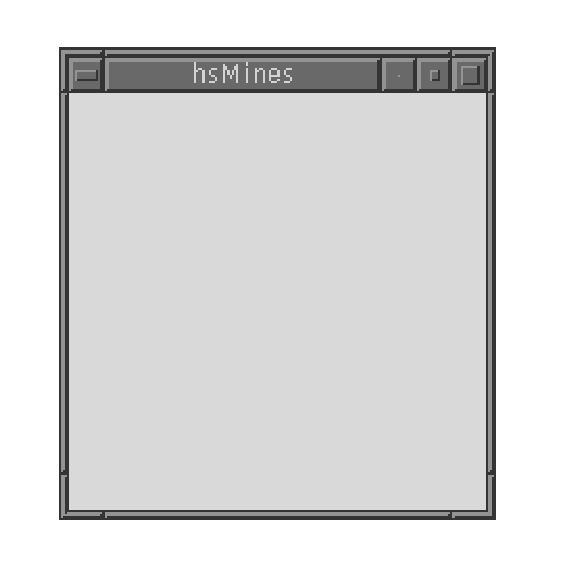
\includegraphics[scale=0.6]{Screenshot1}
\caption{The hsMines window}
\end{center}
\end{figure}

The last line is necessary to clean up all the events we've kicked
loose so far.

\subsection{Menus}

What wolud a GUI be without them? Somewhat empty as it seems. So let's
create some menus.

\begin{code}
    menubar <- createMenu main False []
    main # menu menubar

    fm <- createPulldownMenu menubar [text "File"]
    b2 <- createMenuCommand fm [text "Restart"]
    restartClick <- clicked b2
    b3 <- createMenuCommand fm [text "Quit"]
    quitClick <- clicked b3

    em <- createPulldownMenu menubar [text "Preferences"]
    _ <- createMenuCommand em [text "Cut"]
    _ <- createMenuCommand em [text "Copy"]
    _ <- createMenuCommand em [text "Paste"]
\end{code}
  
First, we create an Menu called menubar inside main, which is our
window. Then we asign menubar as main's menu. That would leave us with
a still rather boring empty menubar.\\
So we create two pulldown menus, called fm an em. Inside these
pulldowns we create a couple of menu commands. The commands in em are
by now just there for the fun of it an not bound to any
variable\footnote{ Don't ask me why commands called Cut, Copy and
  Paste are in a menu called Preferneces. First of all I'm just
  writing the text, not the source. Second is, that these commands are
  not bound to a variable eitherway so you could call them Huey,
  Dewey, and Louie if you prefer that.}.
So let's switch our focus to menu fm. There we create two commands
bound to b2 and b3. And for later use these variables are bound via an
Event to some other Event. We will come to this later. By now the GUI
looks like this:

\begin{figure}[h]
\begin{center}
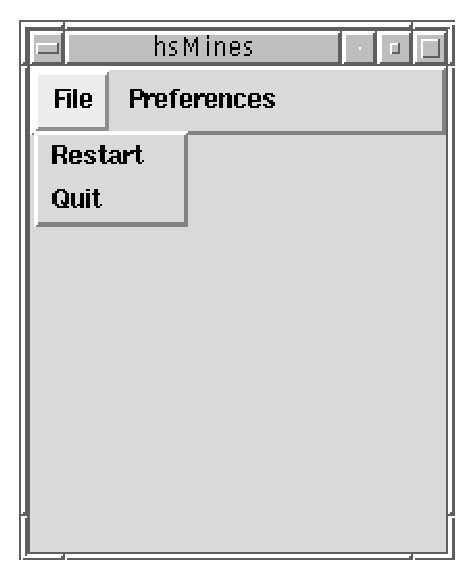
\includegraphics[scale=0.6]{Screenshot2}
\caption{The hsMines main window with an open File menu}
\end{center}
\end{figure}

\subsection{The field}

To make all the decoration perfect, wie need the little smiley atop
the playfield which can be used to restart the game.
\begin{code}
    sm <- newButton main [text ":-)"]
    restart2Click <- clicked sm

    pack sm [Side AtTop, PadY 20, PadX 20, Anchor North] 
\end{code}
So we create a Button called sm (from \textbf{sm}iley btw) and bind it
to another Event. And because the GUI does not automaticaly know where
and when to place the button we have to tell it to \texttt{pack sm at
  the top of the main window, pad it 20 pixels wide in any direction
  and keep it align to the upperside} (which is North on most maps).

\begin{figure}[h]
\begin{center}
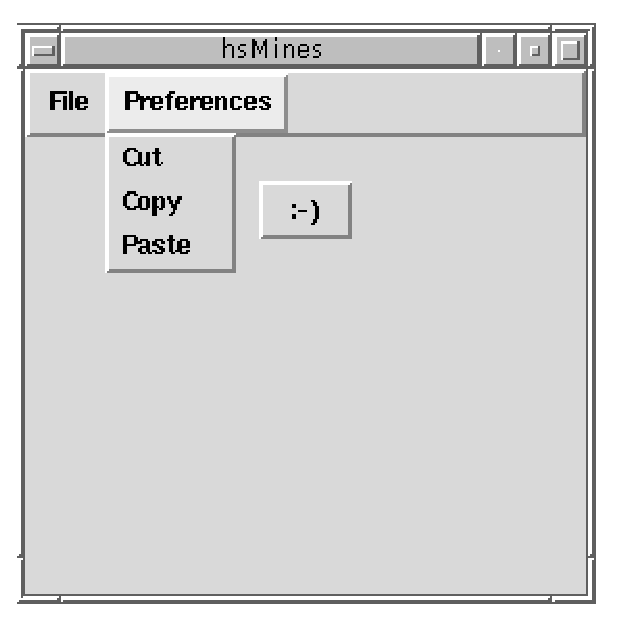
\includegraphics[scale=0.6]{Screenshot3}
\caption{The hsMines main window with smiley}
\end{center}
\end{figure}

I also opened the second menu so you could see Huey, Dewey and
Louie\dots

\begin{code}
    restartCh <- newChannel

    let size= (20, 20)

    bfr <- newFrame main [width (cm 10)]
    allbuttons <- buttons bfr sm (receive restartCh) size 

    pack sm [Side AtTop, PadY 20, PadX 20, Anchor North]

    pack bfr [Side AtTop, PadX 15] 
    mapM_ (\(xy, b)-> grid b [GridPos xy]) allbuttons
    
    -- start the menu handler
    spawnEvent (forever (restartClick >>> sendIO restartCh ()
                      +> restart2Click >>> sendIO restartCh ()
                      +> quitClick >>> destroy main))

\end{code}
To get it realy started we create an IO-channel named restartCh. Then
we create a new Frame (a container widget) with a fixed width and do
somethin strange about allbuttons. Of course this is not that strange.
A function (buttons) is called with some complex arguments and the
result is asigned to allbuttons. We will cover this just some lines
later.

The Frame is packed below the smiley button. They both are told to be
at the top of main, but because only one of them can be there they're
placed below each other in packing order.

To have something to happen with the buttons an Event is spawned. This
single Event listens to some GUI Events we bound some of our buttons
to. Whenever (the Events last until the destruction of the main
thread) one of these three Events occurs, a function is called. The
smiley button and the restart command in the File menu both send an IO
command via the initialised IO channel, the quit command initiates the
destruction of the window and thereby the main thread. If this
happens, finishHTk at the end of the source is reached and the garbage
collection can free all used RAM. But if we don't press one of the
restart buttons, nothing will happen with the many buttons we created
and they all just show a question mark.

\begin{figure}[h]
\begin{center}
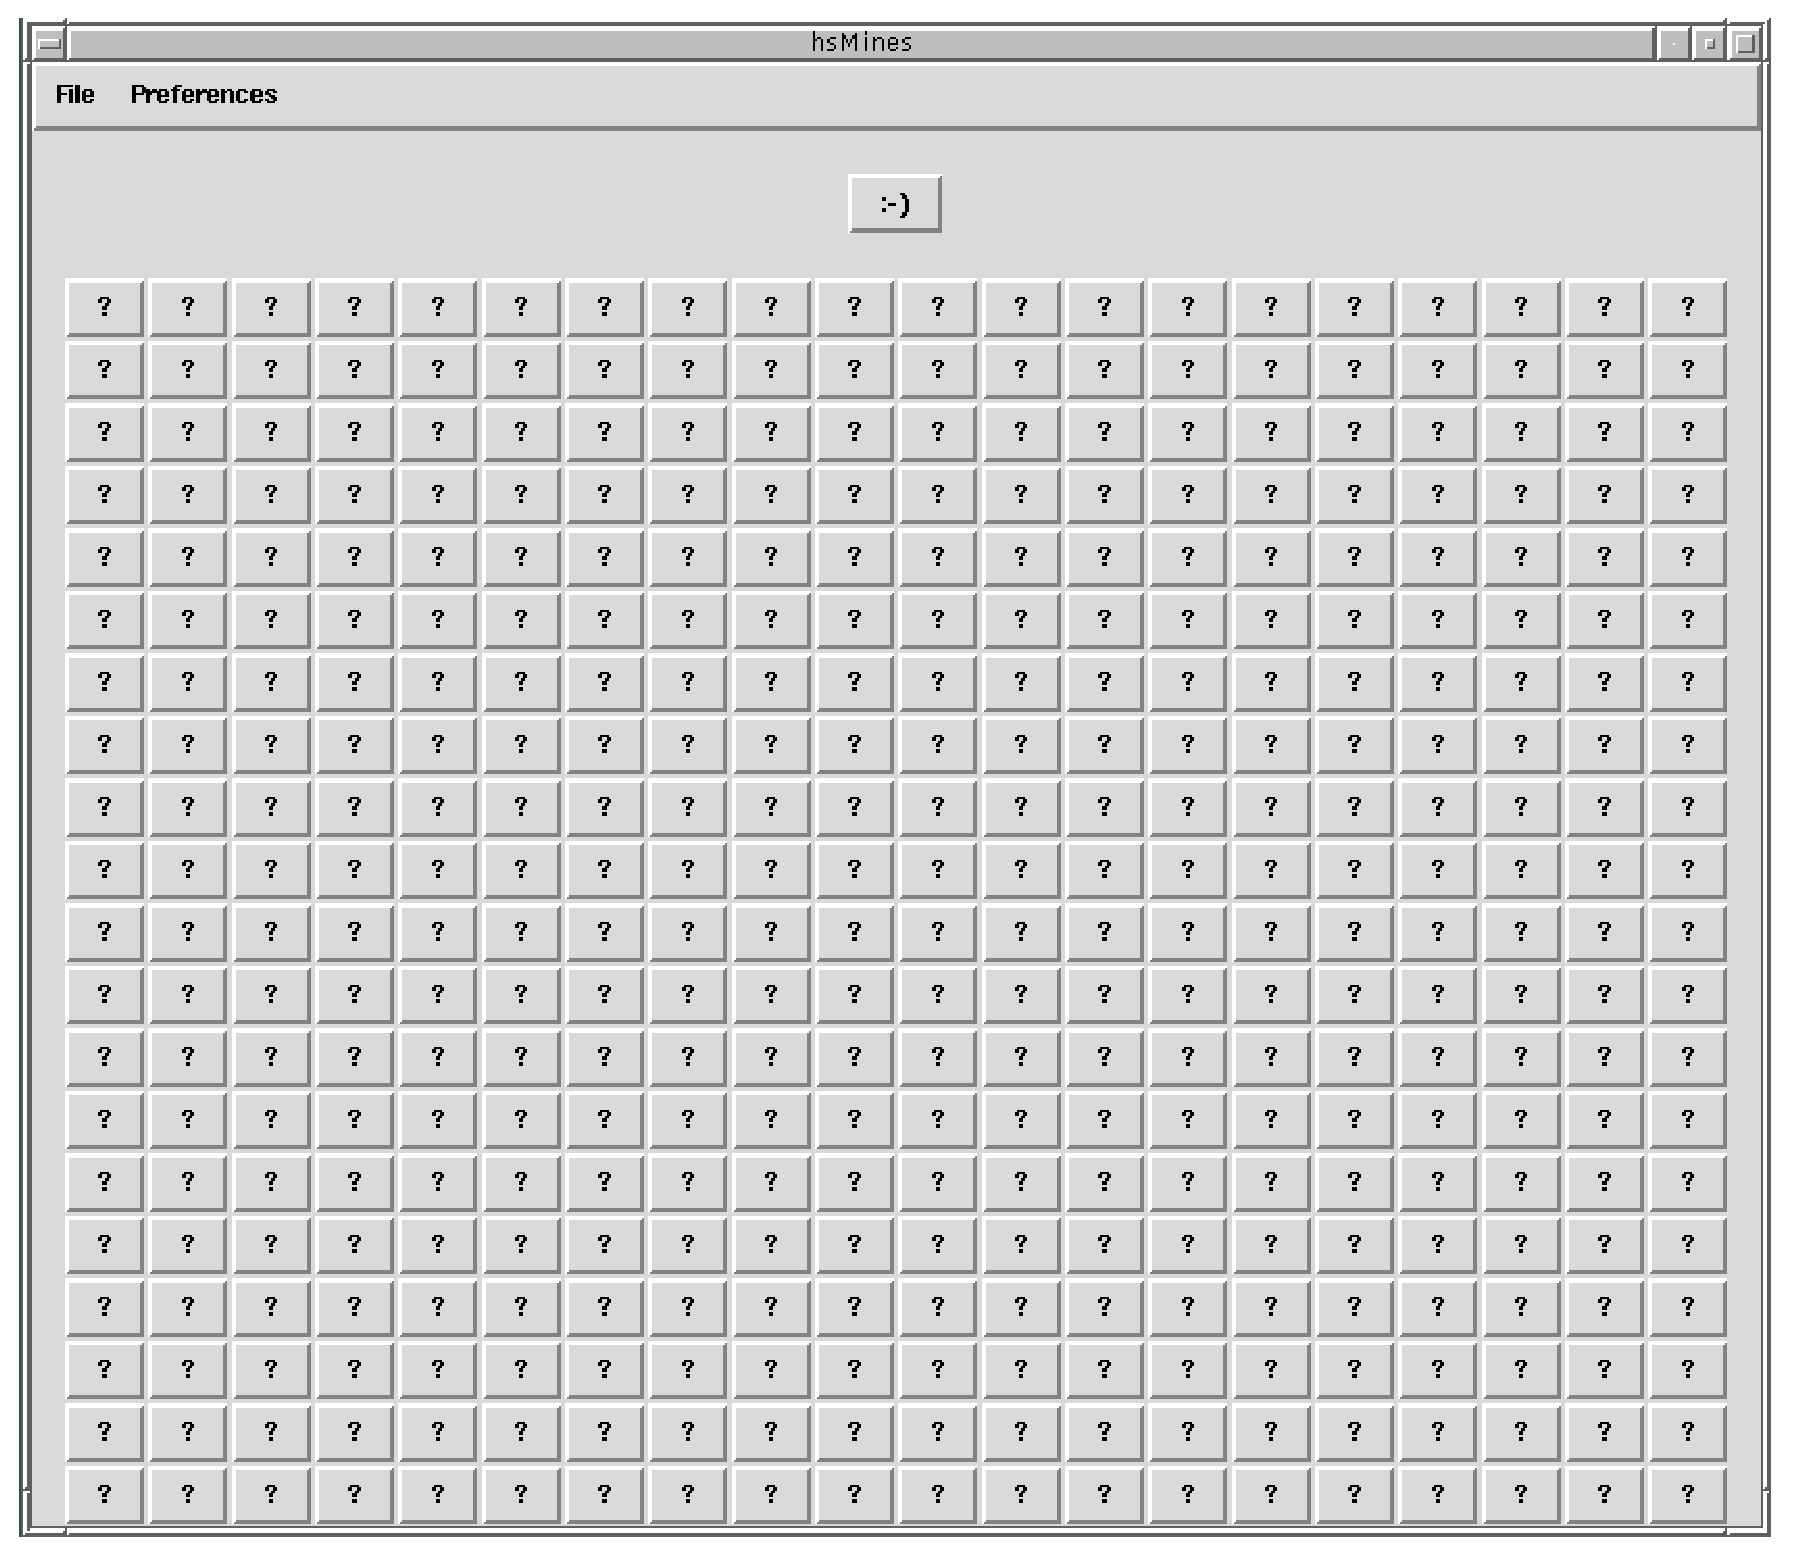
\includegraphics[scale=0.2]{Screenshot4}
\caption{The uninitialised playfield of hsMines}
\end{center}
\end{figure}

So all that is left to do in the main function is to initiate the game
for the first time.

\begin{code}
    sendIO restartCh ()
\end{code}

That's all so far. But as you allready know, something happens to
allbuttons in between.

\subsection{The buttons function}

This function has a rather complex signature.

\begin{code}
buttons :: Container par=> par-> Button-> Event() -> (Int, Int)
                           -> IO [((Int, Int), Button)]

\end{code}

For comparison lets have another look on how it's called:

\begin{code}
    allbuttons <- buttons bfr sm (receive restartCh) size   
\end{code}

We have a class restriction on the first argument, par, which has to
be a container. par happens to be just that, a Frame. Lucky us. The
next argument has to be a button as we can happily admit our smiley
buttons is. The third argument has to be an Event. This Event occurs,
when some IO() is send via the IO Channel restartCh and is received by
receive. The last argument is a 2-tuple of Int which is the size of
the game field. Because size is a function with no arguments (thereby
it's a constant value), the field's size can not be changed.

%An dieser Stelle k�nnte man doch eigentlich wunderbar das Menu
%Preferences ins Spiel bringen und eine Reihe von Auswahlgr��en (aka
%Schwierigkeitsleveln) einbauen, oder?

When buttons has done it's work, it will return an IO of a list auf
tuples of tuples of Int an a Button. As you see it is simpler to watch
the signature yourself than to try to puzzle out what I just told you.

The code of buttons is simple a start.


\subsubsection{Create an array of buttons,\dots}

\begin{code}
buttons par sb startEv (size@(xmax, ymax)) =
  do buttons <- mapM (\xy-> do b<- newButton par [text "?"]
                               return (xy, b)) [(x, y) | x <- [1.. xmax],
                                                         y <- [1.. ymax]]
\end{code}

This code is executed no matter what startEv might be! It creates all
the buttons and writes a quotationmark inside so the playfield looks
the way the Figure above shows it.%Verweis auf Figure?
But there is more to happen in the buttons function!


\subsubsection{bind them\dots}

\begin{code}
     let bArr = array ((1,1), size) buttons
         getButtonClick b n xy = 
            do (click, _) <- bindSimple b (ButtonPress (Just (BNo n)))
               return (click >> return xy)
     leCl <- mapM (\(xy, b)-> getButtonClick b 1 xy) buttons
     riCl <- mapM (\(xy, b)-> getButtonClick b 3 xy) buttons
\end{code}

This looks rather complicated but does nothing more than what we did,
when we bound the smiley button to the restart2Click Event. It's just
that we bind the whole Array of buttons we created via a slightly
adjusted Event (\texttt{getButtonClick b 1/3 xy})\footnote{
  As you could surely guess, 2 would be the modifier to get the center
  button bound.
} to two Events.


\subsubsection{and start\dots}

\begin{code}
     spawnEvent start
     return buttons
\end{code}

At the end, we spawn an Event called start and wait. But wait what
for? As you remember an Event is handed over to buttons. And this
event is used to get the game finaly running.

\begin{code}
         start :: Event ()
         start = startEv >>> do m <- createMines (snd (bounds bArr))
                                mapM_ (text " ") (elems bArr)
                                sb # (text ":-)")
                                sync (play m)
\end{code}

This says: If the Event start occurs (by being spawner for example)
and if startEv is the same kind of Event as start (and occurs at the
same time, that is), we execute some more code. Have a look on how we
create mines later, it's of no importance for the GUI. We map over all
elements in the button array and write `` '' to their text. Then we
asign a new smiley to the text of sb (mapM\_ does the same to all the
buttons) and synchronize the start Event to the play Event. No new
Event is created, start just changed into play.

\subsubsection{to play\dots}

\begin{code}
         play :: Mines-> Event ()
         play m = do r <- choose leCl >>>= open bArr m
                     case r of Nothing -> always gameLost >> gameOver
                               Just nu -> play nu
                  +>
                  do r<- choose riCl >>>= flag bArr m
                     play r
                  +>
                  start 
\end{code}

Playing is easy. To play with a set m of mines means to execute three
steps over and over again.

\begin{enumerate}
\item If the left mousebutton is pressed, execute open with the
  button array and the mines. If nothing is left, you loose. If there
  are mines left, you play on.
\item If the right mousebutton is pressed, execute glag with the
  button array and the mines. No evil may occur, just play on.
\item If thing go awry, goto start and wait for the startEv Event.
\end{enumerate}


\subsubsection{until it's over.}

gameLost is just an alert Window to open, to tell you that you've
lost that also changes your smiley into a freak. You are allowed to
kill the messenger.

\begin{code}
         gameLost :: IO ()
         gameLost = do createAlertWin "*** BOOM!***\nYou lost." []
                       sb # (text "X-(")
                       done
\end{code}

Only after you finished up the messenger, the game is realy over, the
\verb�>>� operator takes care of that.

\begin{code}
         gameOver :: Event ()
         gameOver = start 
                    +> 
                    (choose (leCl++ riCl) >> gameOver) 
\end{code}

gameOver is the Event to take over. It leads you back to the start
event, waiting for the startEv Event to occur. If any of the ingame
Events occur, because some dumbhead did not understand the "`BOOM! You
lost."' message or what so ever, the game is still over and nothing
changes.

That's it, anything else is just plain haskell. Naugh, you're right,
there is some tiny tidbits left. Nobody explained how the numbers show
up when an non mine field is explored, right? Okay, we'll come to that
now.

\subsection{Fuzzing around on the play field}




%%% Local Variables: 
%%% mode: latex
%%% TeX-master: "intro"
%%% End: 

